% https://ida2021.org/regular-paper-track/
% https://www.springer.com/gp/computer-science/lncs/conference-proceedings-guidelines
% Submission website: https://easychair.org/conferences/?conf=ida2021

% This is samplepaper.tex, a sample chapter demonstrating the
% LLNCS macro package for Springer Computer Science proceedings;
% Version 2.20 of 2017/10/04
%
\documentclass[runningheads]{llncs}

\usepackage[
	backend=biber,
%	style=authoryear-icomp,
	sortlocale=en_US,
	natbib=true,
	url=false, 
	doi=true,
	eprint=false
]{biblatex}
\addbibresource{../../bib_file_THESIS.bib}

\usepackage[utf8]{inputenc}
\usepackage[T1]{fontenc}

%
\usepackage{graphicx}
% Used for displaying a sample figure. If possible, figure files should
% be included in EPS format.
%
% If you use the hyperref package, please uncomment the following line
% to display URLs in blue roman font according to Springer's eBook style:
% \renewcommand\UrlFont{\color{blue}\rmfamily}

%\usepackage{amsthm}
%\usepackage{amsfonts}
\usepackage{marvosym, amssymb, mathtools} % Mathesachen
%\usepackage{amstext}
%\usepackage{amsmath}
%\usepackage{siunitx} %Schöne Darstellung großer Zahlen \num{}
%\usepackage{mathpazo} % Palatino für Mathemodus
\usepackage{bbold} % for \mathbb{1}
\usepackage{xfrac} % for \sfrac
\usepackage{csquotes} % for \enquote

\usepackage{tikz,pgfplots,pgf}

\newcommand{\eye}{\mathbb{1}} % Identitiy matrix
\newcommand{\one}{\textbf{1}} % One-vector (1 1 ... 1)
\newcommand{\IN}{\mathbb{N}} % Natural numbers
\newcommand{\IP}{\mathbb{P}} % Prime numbers
\newcommand{\IR}{\mathbb{R}} % Real numbers
\newcommand{\IZ}{\mathbb{Z}} % Integers
\newcommand{\IQ}{\mathbb{Q}} % Rational numbers
\newcommand{\ID}{\mathbb{D}} % Dyadic numbers
\newcommand{\IC}{\mathbb{C}} % Complex numbers
\newcommand{\IF}{\mathbb{F}} % (Vector) Field

\newcommand{\mset}[1]{\{\mskip-5mu\{{#1}\}\mskip-5mu\}}
\newcommand{\Mset}[1]{\big\{\mskip-5mu\big\{{#1}\big\}\mskip-5mu\big\}}
\newcommand{\BigMset}[1]{\Big\{\mskip-5mu\Big\{{#1}\Big\}\mskip-5mu\Big\}}

\newcommand{\amax}[1]{\operatorname*{argmax}_{#1}}

%%% Pseudocode
\usepackage[ruled]{algorithm}
\usepackage[noend]{algpseudocode} 
\makeatletter
\def\BState{\State\hskip-\ALG@thistlm}
\algdef{SE}[DOWHILE]{Do}{DoWhile}{\algorithmicdo}[1]{\algorithmicwhile\ #1}
\makeatother
% !TeX spellcheck = en_US

\begin{document}
%

\title{Learning graph similarity measures using the Weisfeiler-Lehman label hierarchy}
%\title{Learning graph similarities by learning a tree metric on the Weisfeiler-Lehman label hierarchy, used as ground distance for the Wasserstein distance between Weisfeiler Lehman vector representations of graphs.}
%
\titlerunning{Learning graph similarity measures}
% If the paper title is too long for the running head, you can set
% an abbreviated paper title here
%
\author{
Fabrice Beaumont%\inst{1}%\orcidID{0000-1111-2222-3333} 
% \and Pascal Welke\inst{1}\orcidID{0000-0002-2123-3781}
}
%
\authorrunning{F. Beaumont} %, P. Welke}
% First names are abbreviated in the running head.
% If there are more than two authors, 'et al.' is used.
%
\institute{University of Bonn, Germany}
%
\maketitle
% typeset the header of the contribution
%
\begin{abstract} % 150--250 words.
In this expose I am outlining the research questions and research strategy of my master thesis. 
In my thesis, I am going to investigate the effect of learning such similarities between Weisfeiler Lehman labels and using these in the definition of a graph similarity measure, structured similarly to the Wasserstein Weisfeiler Lehman graph kernel proposed in 2019 by Togninalli et al.
The goal is to discuss, whether learning such similarities can improve the flexibility of the resulting graph similarity measure.
The machine learning will be restricted in the sense that the ground distance is set as a a tree metric on the Weisfeiler Lehman label hierarchy tree. 
The learning procedure is to iteratively update the edge weights in this tree and thus to change the resulting distance between the Weisfeiler-Lehman labels used.

\keywords{Weisfeiler Lehman \and Tree Metric \and Graph Classification \and Metric Learning \and Wasserstein distance\dots.}
\end{abstract}

%TODO: Use the GOT Optimal Transport paper. Reference its results? Is it cited by the other ones? And use its introductioni on similarity measures and why to use the Wasserstein Distance, and why it cannot be differentiated.

\section{Introduction} \label{sec:Introduction}
Digitization is rapidly increasing the amount of digitally stored data.
Such data is often represented by graphs, which may capture potentially complex structures.
Common examples of such data storing graphs are social and sensor networks, program flows and structures in chemo- and bio-informatics (e.g. molecules, proteins, genes and chemical compounds). 
Based on functional properties of the graphs one may define classifications on them. 
To extend the classification of known graph instances to unknown instances is one of many different challenges when working with such graph data. 
Such classification can indicate, for example, whether a particular molecule can trigger mutations or not. 
In this framework it is usually assumed, that graphs with similar structure have similar properties and therefore should be classified similarly.
Therefore, it is important to quantify the similarity between graphs~\cite{2011_Shervashidze_JMLR}. 
Due to the lack of efficient similarity measures between graphs, the analysis, classification and prediction of graph data stays challenging.

The most sensitive similarity measure is the binary decision whether two given graphs are isomorphic (topologically identical) or not.
%The computation of this measure is in NP~\cite{1979_Garey_BOOK}. 
%Furthermore, the task of testing weather for two given graphs one is isomorphic to a subgraph of the other one, is NP-complete~\cite{1979_Garey_BOOK}. 
%And the seemingly reasonable approach to restrict the isomorphism test to a unique subgraph, like the largest common subgraph, is of limited use, since finding such largest common subgraphs is a NP-complete problem, as well~\cite{1979_Garey_BOOK}.
There are several different approaches to defining a more sophisticated similarity measure.
Some examples are measures based on the graph edit distance~\cite{1983_Bunke_ELSEVIER,2005_Froehlich_ICML}, optimal assignment kernels~\cite{2005_Froehlich_ICML}, the
skew spectrum~\cite{2008_Kondor_ICML} or the graphlet spectrum~\cite{2009_Kondor_ICML,2009_Shervashidze_NIPS}. %TODO: Verify the connections of the papers to the written text
In the context of similarity measures, graph kernels have the desirable property of enabling the application of a larger toolbox of kernelized learning methods on graph-structured data.
% pioneer work on convolution kernels over discrete structures \cite{1999_Haussler_CONF} (formulated as such in the introduction in \cite{2021_Schulz_CONF})

By restricting the kernels to substructures of graphs, they can be computed in polynomial time~\cite{2008_Hofmann_CONF}. 
This restriction however may at the same time limit their ability to capture complex characteristics of the graphs. 
That is why most proposed variants do not generalize well to graphs with high-dimensional continuous vertex attributes~\cite{2011_Shervashidze_JMLR}. 
In 2019, Togninalli et al. established their Wasserstein Weisfeiler-Lehman (WL) Graph Kernels as the new state of the art.
These kernels are capable of processing both categorical labels and continuous attributes by utilizing the the Hamming distance and Euclidean distance as ground metric for the Wasserstein distance~\cite{2019_Togninalli_NIPS}.
However, these rigid, rather arbitrary definition does not permit to adjust the distances between the labels (or attributes) used in the graph.
This may be disadvantageous, since the labels constructed by the WL labeling scheme represent entire substructures, also known as unfolding trees~\cite{2021_Schulz_CONF}.
In its naive version, two labels are distinguished as either equal or different.
But since the substructures, that they represent, can differ largely or only little, 
a more nuanced differentiation may be appropriate.
To do so, I introduce adjustable distances between the labels.
These can also be useful to introduce-application specific knowledge about the similarity of the original labels (or attributes) or even whole substructures. 
Since such application-based differences may not be known or only partially known, one may try to use machine learning to find such database-specific distances. 
If this is possible, the learned distances could potentially reveal unknown application-based knowledge on the substructures of the used graphs. 

In my masters thesis I am going to investigate, how well a measure for similarity can be learned, based on a similarity definition using the WL-labeling hierarchy. 
The structure of the similarity measure is a Wasserstein distance between the WL-label distribution (WL-features) of two given graphs. 
The ground distance of the Wasserstein distance is defined as a tree metric on the WL-labels. 
Thus it highly depends on the edge weights in the hierarchy tree. 
The research question is, if it is possible to learn how to adjust these edge weights, in order to yield a better similarity measure, compared to a static ground distance definition. 
The usage of the Wasserstein distance is motivated by Togninalli et al., who successfully used it to construct a similarity measure for graphs with both categorical vertex labels and continuous vertex attributes~\cite{2019_Togninalli_NIPS}.
As they mention, optimal transport had been used successfully to tackle the graph alignment problem before~\cite{2019_Xu_CONF}.
%
%Before giving details of the used method in section \ref{sec:method} we take an overview about related work in section \ref{sec:related_work}.

\section{Related work}\label{sec:related_work} %TODO: THIS CHAPTER

XY proposed spectral distances as graph similarity measures, which focus on the Laplacian matrix eigenvectors~\cite{2012_Jovanovic_ELSEVIER, 2018_Gera_Springer}.

Maretic et al. proposed a framework for graph similarity measures based on the Wasserstein distance for comparing vector representations of entire graphs~\cite{2019_Maretic_CONF}.
%TODO: Maybe include other - non kernel approaches from the related work section from ~\cite{2019_Maretic_CONF} here

Many graph kernels can be categorized as $\mathcal{R}$-convolution kernels~\cite{2019_Togninalli_NIPS}. 
That is, they define similarity in terms of aggregation of local similarity.
The local similarity is computed between mutual substructures such as 
walks~\cite{2003_Gaertner_CONF,2003_Kashima_ICML}, paths~\cite{2005_Borgwardt_IEEE}, limited-size subgraphs like graphlets~\cite{2004_Horvath_KDD,2009_Shervashidze_NIPS}, subtree patterns~\cite{2003_Ramon_CONF,2008_Mahe_CONF,2011_Shervashidze_JMLR} or combinations of them. % This grouping is roughly supported in \cite{2021_Schulz_CONF,2019_Shervashidze_NIPS}
One important example for such a combination is the General WL kernel proposed by Nino Shervashidze et. al~\cite{2011_Shervashidze_JMLR}. 
This kernel is based on the WL labels and can be combined with any other
graph kernel (base kernel), since it simply sums up the base kernels results for every WL label iteration. 
The authors themselves present a subtree, edge and shortest path variation in their paper “Weisfeiler-Lehman Graph Kernels”~\cite{2011_Shervashidze_JMLR}. 
%The method which shall be investigates in my master thesis, the Laplacian kernel is based on the distance matrix of the graphs which is computed on one WL labeling iteration.
%But adding the distances of multiple WL-labeling iterations (that is to used the constructed WLLT completely) is equivalent to multiplying multiple Laplacian kernels based on the distance matrices for these WL labeling iterations.

%TODO: Integrate or move to Research
Later work has moved away from solely counting equivalent substructures~\cite{2021_Schulz_CONF}.
- Compute optimal assignment between vertices~\cite{2016_Kriege_NIPS}
- Compute optimal transport as a form of 'soft-matching' between vertices~\cite{2019_Togninalli_NIPS}
- Neighborhoods as Rooted DAG %TODO> G. D. S. Martino, N. Navarin, and A. Sperduti. A tree-based kernel for graphs. In SIAM SDM, pages 975–986, 2012.

\section{Framework and definitions}\label{sec:definitions} %TODO: THIS CHATPER

Before describing the details of the proposed method, let me introduce some basic definitions. 
An (undirected) graph is a tuple $G = (V, E)$ where $V$ is a finite set of vertices and $E\subseteq 2^V$ is a finite set of undirected edges on them.
$G$ is called labeled, if there exists a vertex labeling function $\ell: V \to\Sigma_V$ for a finite label alphabet $\Sigma$.
%$G$ is called attributed, if there exists a vertex attribute function $a: V \to\IR$.
The labels can be included in the definition of the graph by writing $G = (V, E, \ell)$. % or $G = (V, E, a)$ respectively.
%When $G$ is clear from the context, denote the number of vertices as $n:=|V|$ and the number of edges as $m:=|E|$.
$G$ is called weighted if there exists an edge-weight function $w:E\to\mathbb{R}$.
Two graphs $G_1$ and $G_2$ are isomorphic ($G_1 \equiv G_2$), if there exists a bijective function between their vertices, that preserves all edges and labels.
For a graph $G = (V, E)$ and a vertex $v\in V$ we call the set $\mathcal{N}^1(v) := \{u \in V |\ (u, v) \in E\}$ the first neighborhood of $v$ in $G$.
The degree $\delta(v)$ of a vertex $v \in V$ is given as the size of its first neighborhood, that is $\delta(v):= |\mathcal{N}(v)|$.
Similarly we define the $d$-th neighborhood (sometimes referred to as $d$-hop neighborhood) of $v$ in $G$ (for $1<d\in\IN$) as the set of all vertices that are not $v$ itself, that can be connected with $v$ by a path of length $d$:
\[ \mathcal{N}^d(v) := \big\{u \in V |\ \exists w\in\mathcal{N}^{d-1}(v) \ \text{s.t.}\ (u, w) \in E\big\}\backslash\{v\} \]
Call $\mathcal{N}_+^d(v) := \mathcal{N}^d(v)\cup\{v\}$ the extended $d$-th neighborhood of $v$ in $G$. 

\subsection{Weisfeiler-Lehman labeling scheme}

The here used Weisfeiler-Lehman labeling scheme is vertex labeling scheme at the center of the Weisfeiler-Lehman test of isomorphism. 
More specifically I will make use of its 1-dimensional variant (also known as 1-WL vertex embedding, WL color refinement, naive vertex refinement or 2-WL as higher-dimensional WL labeling scheme)~\cite{2011_Shervashidze_JMLR, 2019_Xu_CONF}. 
The scheme iteratively propagates neighborhood information by compressing this information in labels and iteratively assigning these to the vertices~\cite{1968_Weisfeiler_CONF}.
We will call such assigned labels WL-labels.
The general WL color refinement is described more formally in algorithm \ref{alg:WLmethod}.
%TODO: What about initial labels. Reference unfolding trees.
%The algorithm proceeds in iterations, which I index by $k$. In each iteration, the current vertex labels are used to define new vertex labels, which then replace them in the next iteration. One iteration comprises the following steps.
\begin{algorithm}[H]
	\caption{WL color refinement} \label{alg:WLmethod} 
	\begin{tabbing}
		\textbf{Output:} \= \kill
		\textbf{Input:} \>a graph $G=(V, E, \ell)$,\\
		\>a perfect hash function $\operatorname{hash}$.\\		
		\textbf{Output:} \>a vector representation of $G$ of size $|V|$.
	\end{tabbing}	
	\begin{algorithmic}[1]
		\State $c(v)^0 \leftarrow \operatorname{hash}(\ell)$ for all $v\in V$
		\While {$\big(c^{k}(v)\big)_{v\in V} \neq \big(c^{k-1}(v)\big)_{v\in V}$}
			\State $c^{k}(v) \leftarrow \operatorname{hash}\big(c^{\ell-1}(v), \mset{c^{k-1}(w)| \ w\in\mathcal{N}_G(v)} \big)$ for all $v\in V$ \label{line:newWlHash}
		\EndWhile		
		\State\Return $\mset{c^{k}(v)| \ v\in V}$
	\end{algorithmic}
	Note that there are several possible implementations of the hash function and the concatenation step in line \ref{line:newWlHash}. % The procedure is generalized in 2019_Xu_CONF
	% $c(v)_0 = \ell(v)$ for labeled graphs and $c(v)_0 = |\mathcal{N}(v)|$ for unlabeled graphs \cite{2009_Shervashidze_NIPS}
\end{algorithm}
% WL graph kernels are conceptually limited to comparing labels with respect to equality. While this comparison is well-suited for graph isomorphim tests, it is too restrictive for defining similarities. \cite{2021_Schulz_CONF}

In algorithm \ref{alg:WLmethod} the color refinement is repeated until the representations do not change, that is until a stable configuration is found. This can be used as an imperfect graph isomorphism test. %TODO> cite
However, for our purposes, an intermediate compression level of the graph structure may be sufficient. 
Thus we add as input the desired number of labeling iterations $k$ and execute the commands in the while-loop $k-1$ times.
The new set of WL-labels in the $i$-th iteration $(V, c^i)$ are called the $i$-th WL-feature of the graph.

Note that after the first iteration, the WL labels encode the information of the labels of the first neighborhood (those reachable with paths of length one).
In the $d$-th iteration, the WL labels encode the information of the labels of the $d$-th neighborhood, since they are constructed on previously defined WL labels, 
which in turn encode information about neighbors that are further away.
%TODO of the neighborhood and the current label
%\textit{Theorem:} Isomorphy invariance of Weisfeiler and Lehman's vertex representation.	Let $G, H$ be two graphs with vertex label functions $r_0^{\text{WL}, G}, r_0^{\text{WL}, H}$. If $G$ and $H$ are isomorphic (respecting $r_0^{\text{WL}, G}$, $r_0^{\text{WL}, H}$) then
%\[ \forall k\ge 0:\qquad \mset{ r_k^{\text{WL}, G}(v)| \ v\in V(G)} =  \mset{ r_k^{\text{WL}, H}(v)| \ v\in V(H)} \]
%This means the vertex representation can reduce the graph isomorphy to multiset equality.\\
%{\ref{thm:WeisfeilerLehmanIsoInv}}
%The proof follows directly from the invariance theorem (theorem \ref{thm:MessagePassingInvariantUnderIsom}) for the message passing framework
%
%Th WL vertex representation is at most as expressive as GNNs... %GRL Script and GIN

\begin{minipage}{\textwidth}
	\begin{figure}[H]
		\centering
		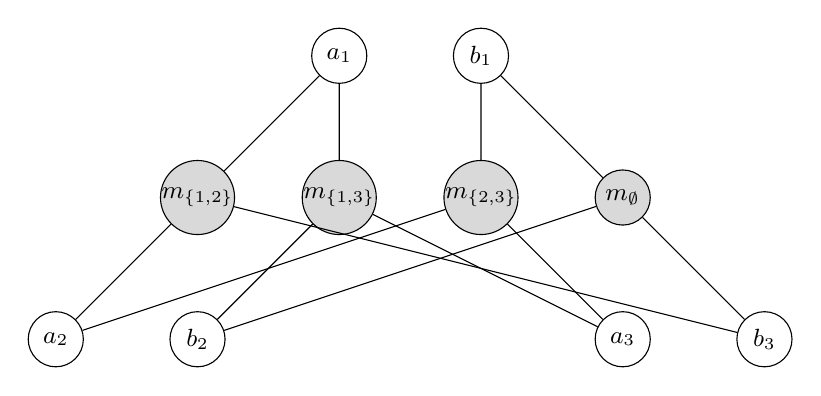
\begin{tikzpicture}[x=2cm,y=2cm] 
		\begin{scope}[scale=0.9]
		
		\tikzstyle{mycircle}=[circle,
		draw=black,
		fill=gray,
		fill opacity = 0.3,
		text opacity=1,
		inner sep=0pt,
		minimum size=7mm,
		font=\small
		]
		\tikzstyle{mycirclewhite}=[circle,
		draw=black,
		text opacity=1,
		inner sep=0pt,
		minimum size=7mm,
		font=\small
		]
		
		\coordinate (pa2) at (0, 0);
		\coordinate (pb2) at (1, 0);
		
		\coordinate (pa1) at (2, 2);
		\coordinate (pb1) at (3, 2);
		
		\coordinate (pa3) at (4, 0);
		\coordinate (pb3) at (5, 0);
		
		\coordinate (pm12) at (1, 1);
		\coordinate (pm13) at (2, 1);
		\coordinate (pm23) at (3, 1);
		\coordinate (pme) at (4, 1);
				
		\node[mycirclewhite] (a2) at (pa2) {$a_2$};
		\node[mycirclewhite] (b2) at (pb2) {$b_2$};		
		
		\node[mycirclewhite] (a1) at (pa1) {$a_1$};
		\node[mycirclewhite] (b1) at (pb1) {$b_1$};
		
		\node[mycirclewhite] (a3) at (pa3) {$a_3$};
		\node[mycirclewhite] (b3) at (pb3) {$b_3$};
		
		\node[mycircle] (m12) at (pm12) {$m_{\{1,2\}}$};
		\node[mycircle] (m13) at (pm13) {$m_{\{1,3\}}$};
		\node[mycircle] (m23) at (pm23) {$m_{\{2,3\}}$};
		\node[mycircle] (me) at (pme) {$m_{\emptyset}$};
		
		
		\draw[-] (a2) -- (m12);
		\draw[-] (a2) -- (m23);
		\draw[-] (b2) -- (m13);
		\draw[-] (b2) -- (me);
		
		\draw[-] (a1) -- (m12);
		\draw[-] (a1) -- (m13);
		\draw[-] (b1) -- (m23);
		\draw[-] (b1) -- (me);
		
		\draw[-] (a3) -- (m13);
		\draw[-] (a3) -- (m23);
		\draw[-] (b3) -- (m12);
		\draw[-] (b3) -- (me);				
		
		\end{scope}
		\end{tikzpicture}
	\end{figure}
	\label{fig:counterExampleWL}
\end{minipage}
$X_3 = (V_3, E_3)$ with $V_3 = A_3 \cup B_3 \cup M_3$ and $A_3 =\{ a_1, a_2, a_3 \}$, $B_3 =\{ b_1, b_2, b_3 \}$, $M_3 =\{ m_{1,2}, m_{1,3}, m_{2,3}, m_{\emptyset} \}$. $E_3$ contains edges $\{ a_i, m_{S} \}$ and $\{ b_j, m_{S} \}$ such that $i\in S$ and $j\neq S$~\cite{1992_Cai_IEEE}. %TODO: compare with source. Write text


\begin{minipage}{.45\textwidth}
	\begin{figure}[H]
		\centering
		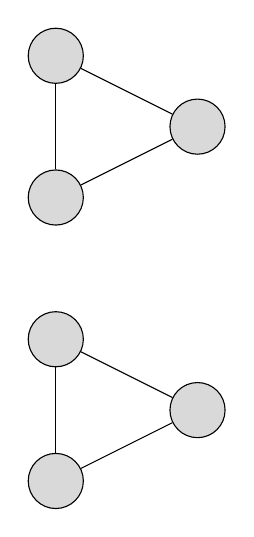
\begin{tikzpicture}[x=2cm,y=2cm] 
		\begin{scope}[scale=0.9]
		
		\tikzstyle{mycircle}=[circle,
		draw=black,
		fill=gray,
		fill opacity = 0.3,
		text opacity=1,
		inner sep=0pt,
		minimum size=7mm,
		font=\small
		]
		\tikzstyle{mycirclewhite}=[circle,
		draw=black,
		text opacity=1,
		inner sep=0pt,
		minimum size=7mm,
		font=\small
		]
		
		\coordinate (pa1) at (0, 3);
		\coordinate (pa2) at (1, 2.5);
		\coordinate (pa3) at (0, 2);
		
		\coordinate (pb1) at (0, 1);
		\coordinate (pb2) at (1, 0.5);
		\coordinate (pb3) at (0, 0);		
						
		\node[mycircle] (a1) at (pa1) {};
		\node[mycircle] (a2) at (pa2) {};
		\node[mycircle] (a3) at (pa3) {};
		
		\node[mycircle] (b1) at (pb1) {};
		\node[mycircle] (b2) at (pb2) {};
		\node[mycircle] (b3) at (pb3) {};		
		
		\draw[-] (a1) -- (a2);
		\draw[-] (a2) -- (a3);
		\draw[-] (a3) -- (a1);
		
		\draw[-] (b1) -- (b2);
		\draw[-] (b2) -- (b3);
		\draw[-] (b3) -- (b1);
		
		\end{scope}
		\end{tikzpicture}
		\caption{$G_1$ - Two disconnected circles, each of length three.}	
		\label{fig:counterExampleWLCai0}
	\end{figure}
\end{minipage}
\begin{minipage}{.45\textwidth}
	\begin{figure}[H]
		\centering
		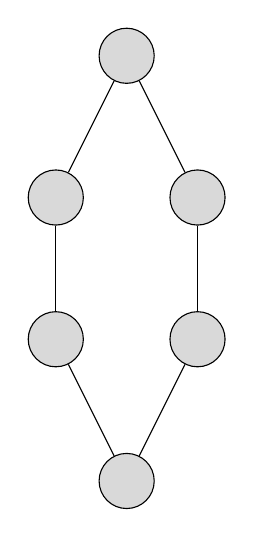
\begin{tikzpicture}[x=2cm,y=2cm] 
		\begin{scope}[scale=0.9]
		
		\tikzstyle{mycircle}=[circle,
		draw=black,
		fill=gray,
		fill opacity = 0.3,
		text opacity=1,
		inner sep=0pt,
		minimum size=7mm,
		font=\small
		]
		\tikzstyle{mycirclewhite}=[circle,
		draw=black,
		text opacity=1,
		inner sep=0pt,
		minimum size=7mm,
		font=\small
		]
		
		\coordinate (pa1) at (0.5, 0);
		\coordinate (pa2) at (0, 1);
		\coordinate (pa3) at (0, 2);		
		\coordinate (pa4) at (0.5, 3);
		\coordinate (pa5) at (1, 2);
		\coordinate (pa6) at (1, 1);		
		
		\node[mycircle] (a1) at (pa1) {};
		\node[mycircle] (a2) at (pa2) {};
		\node[mycircle] (a3) at (pa3) {};		
		\node[mycircle] (a4) at (pa4) {};
		\node[mycircle] (a5) at (pa5) {};
		\node[mycircle] (a6) at (pa6) {};		
		
		\draw[-] (a1) -- (a2);
		\draw[-] (a2) -- (a3);
		\draw[-] (a3) -- (a4);
		\draw[-] (a4) -- (a5);
		\draw[-] (a5) -- (a6);
		\draw[-] (a6) -- (a1);
		
		\end{scope}
		\end{tikzpicture}
		\caption{$G_2$ - A circle of length six.}	
		\label{fig:counterExampleWLCai1}
	\end{figure}		
\end{minipage}

Consider two graphs $G_1$ and $G_2$ (as sketched in figures  \ref{fig:counterExampleWLCai0} and \ref{fig:counterExampleWLCai1}) on six vertices. $G_1$ consists of two disconnected circles each of length three. $G_2$  is a circle of length six. Given no initial labels, the WL labeling scheme considers all vertices equally labeled. Since every vertex in both graphs has exactly two neighbors (with the same label), every vertex will be assigned the same WL-label in the next iteration. The obtained labeling is equivalent to original case, and no number of WL-iterations will generate a different outcome. In this case, the WL-labeling scheme would wrongfully declare the two graphs to be isomorphic. %TODO: mention ~\cite{1992_Cai_IEEE} or not?

\subsubsection{Remarks on the implementation}

When applied to labeled graphs (with a finite set of labels), the labeling scheme can be implemented using integers as WL-labels and with simple perfect hash functions. 
The method can be implemented as an efficient matrix vector multiplication between the adjacency matrix and the WL-label vector using logarithms of prime numbers as WL-labels.

\subsubsection{Implementation as matrix vector multiplication}

The naive implementation of the WL-labeling scheme requires to aggregate the WL-labels in the neighborhood of each vertex, combine this aggregation with the WL-label of the vertex itself and hash it to obtain a new WL-label (with a perfect hash function). 
To obtain a maximally powerful embedding, the aggregation and hashing must be injective~\cite{2019_Xu_CONF}. 
This aggregation is often realized by sorting the WL-labels of the neighborhood first.
By design, the labeling scheme only requires information about the neighborhoods (adjacency matrix) and the WL-labels of the last iteration in order to compute the next WL-labels (containing information about a neighborhood or larger degree).
This can intuitively be understood as a recursive matrix-vector multiplication.
Given the fixed adjacency matrix $A\in\{0,1\}^{|V|}$, the goal is to define WL-labels (WL-features) $w_i \in \IR^{|V|}$ such that the multiplication $A w_i$ leads to the next WL-labels $w_{i+1}$.
This way, the new WL-labels are computed purely as an addition of the old WL-labels.
Using any numbers is not injective, since addiction is not an injective function.
One may think of prime numbers for the WL-labels, since these are at least injective with respect to multiplication.
To get from addiction to multiplication one can use the (injective) logarithm of prime numbers.
Thus the proposed method goes as follows:
Map the original $n$ vertex labels (or attributes) to the logarithms of the first $n$ prime numbers. With original labels given by $\ell_0:V\to[n]$ and prime numbers $p_i\in\IP$ this can be written as: 
\[ \forall v: \ell_0(v) \mapsto \log(p_{\ell_0(v)}) =: \ell_1(v) \]
Now, the $1$-th WL-labels can be computed as
\[ \ell^{\prime}_{1}(\overleftarrow{v}) := \pi\ell_{0}(\overleftarrow{v}) + A \;\ell_{0}(\overleftarrow{v}) = (A+\pi\mathbb{1}) \ell_{0}(\overleftarrow{v})\]
The factor $\pi$ can be replaced by any transcendent number.
It ensures that in the computation of the new label for a vertex $v$ the old label is differentiated from the labels of the neighborhood.
Consider for example a vertex with WL-label $2$ and two neighboring vertices with labels $3$.
If the old labels are not differentiated from the labels of the neighborhood, the vertex with label $2$ in this example would obtain the same label as a vertex with label $3$ and two neighboring vertices with labels $2$ and $3$.
To ensure injectivity of the multiplication, $\ell^{\prime}_{1}$ needs to return prime numbers.
With each iteration the used label values are getting bigger.
This their logarithms may have less and less difference, which could lead to practical problems due to the limited machine precision.
Thus repeat the mapping step between the matrix-vector multiplications to use the logarithm of a prime number for each new WL-label.

\begin{minipage}{\textwidth}
	\begin{figure}[H]
		\centering
		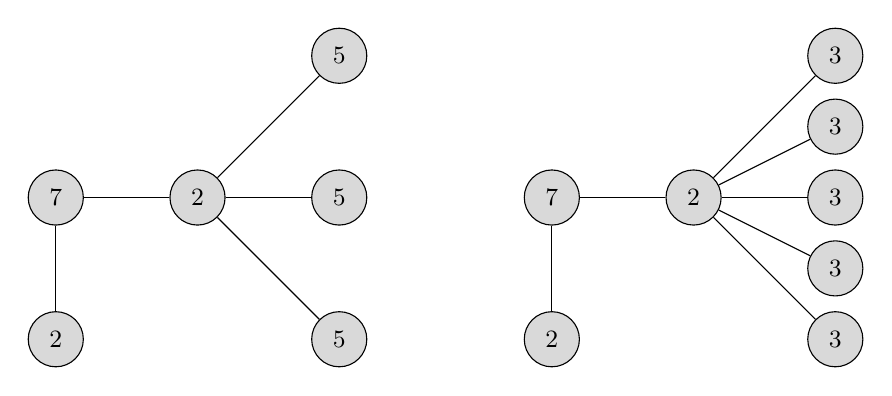
\begin{tikzpicture}[x=2cm,y=2cm] 
		\begin{scope}[scale=0.9]
		
		\tikzstyle{mycircle}=[circle,
		draw=black,
		fill=gray,
		fill opacity = 0.3,
		text opacity=1,
		inner sep=0pt,
		minimum size=7mm,
		font=\small
		]
		\tikzstyle{mycirclewhite}=[circle,
		draw=black,
		text opacity=1,
		inner sep=0pt,
		minimum size=7mm,
		font=\small
		]
		
		\coordinate (pa0) at (-1, -1);
		\coordinate (pa1) at (-1, 0);
		\coordinate (pa2) at (0, 0);
		\coordinate (pa3) at (1, 1);
		\coordinate (pa4) at (1, 0);
		\coordinate (pa5) at (1, -1);
		
		\coordinate (pb0) at (2.5, -1);
		\coordinate (pb1) at (2.5, 0);
		\coordinate (pb2) at (3.5, 0);
		\coordinate (pb3) at (4.5, 1);
		\coordinate (pb4) at (4.5, 0.5);
		\coordinate (pb5) at (4.5, 0);
		\coordinate (pb6) at (4.5, -0.5);
		\coordinate (pb7) at (4.5, -1);
		
		\node[mycircle] (a0) at (pa0) {$2$};
		\node[mycircle] (a1) at (pa1) {$7$};		
		\node[mycircle] (a2) at (pa2) {$2$};
		\node[mycircle] (a3) at (pa3) {$5$};
		\node[mycircle] (a4) at (pa4) {$5$};
		\node[mycircle] (a5) at (pa5) {$5$};
		
		\node[mycircle] (b0) at (pb0) {$2$};
		\node[mycircle] (b1) at (pb1) {$7$};
		\node[mycircle] (b2) at (pb2) {$2$};
		\node[mycircle] (b3) at (pb3) {$3$};
		\node[mycircle] (b4) at (pb4) {$3$};
		\node[mycircle] (b5) at (pb5) {$3$};
		\node[mycircle] (b6) at (pb6) {$3$};
		\node[mycircle] (b7) at (pb7) {$3$};
		
		\draw[-] (a0) -- (a1);
		\draw[-] (a1) -- (a2);
		\draw[-] (a2) -- (a3);
		\draw[-] (a2) -- (a4);
		\draw[-] (a2) -- (a5);
		
		\draw[-] (b0) -- (b1);
		\draw[-] (b1) -- (b2);		
		\draw[-] (b2) -- (b3);
		\draw[-] (b2) -- (b4);
		\draw[-] (b2) -- (b5);
		\draw[-] (b2) -- (b6);
		\draw[-] (b2) -- (b7);	
		
		\end{scope}
		\end{tikzpicture}
	\end{figure}
	\label{fig:exampleForPrimeNrWL}
\end{minipage}

The adjacency matrices below list the vertices in the order from bottom left to top right (with labels $2$, $7$, $2$ and then the vertices with label $5$ or $3$).
\begin{flalign*}
	\begin{bmatrix}
	1 & 1 & . & . & . & . \\
	1 & 1 & 1 & . & . & . \\
	. & 1 & 1 & 1 & 1 & 1 \\
	. & . & 1 & 1 & . & . \\
    . & . & 1 & . & 1 & . \\
    . & . & 1 & . & . & 1 \\
\end{bmatrix} \log\begin{bmatrix}
2 \\ 7 \\ 2 \\ 5 \\ 5 \\ 5
\end{bmatrix} &= \begin{bmatrix}
\log(2)+\log(7) \\ \log(7)+\log(2)+\log(2) \\ \log(2)+\log(7)+\log(5)+\log(5)+\log(5) \\ \log(5)+\log(2) \\ \log(5)+\log(2) \\ \log(5)+\log(2)
\end{bmatrix} \\
	&= \begin{bmatrix}
\log(2*7) \\ \log(7*2^2) \\ \log(2*7*5^3) \\ \log(5*2) \\ \log(5*2) \\ \log(5*2)
\end{bmatrix} \qquad \begin{matrix*}[l]
2|7 \\ 7|2,2 \\ 2|7,5,5,5 \\ 5|2 \\ 5|2 \\ 5|2
\end{matrix*} \\
	\begin{bmatrix}
	1 & 1 & . & . & . & . & . & . \\
	1 & 1 & 1 & . & . & . & . & . \\
	. & 1 & 1 & 1 & 1 & 1 & 1 & 1 \\
	. & . & 1 & 1 & . & . & . & . \\
	. & . & 1 & . & 1 & . & . & . \\
	. & . & 1 & . & . & 1 & . & . \\
	. & . & 1 & . & . & . & 1 & . \\
	. & . & 1 & . & . & . & . & 1 \\
	\end{bmatrix} \log\begin{bmatrix}
	2 \\ 7 \\ 2 \\ 3 \\ 3 \\ 3 \\ 3 \\ 3
	\end{bmatrix} &= \begin{bmatrix}
	\log(2*7) \\ \log(7*2^2) \\ \log(2*7*3^5) \\ \log(3*2) \\ \log(3*2) \\ \log(3*2) \\ \log(3*2) \\ \log(3*2)
	\end{bmatrix} \qquad \begin{matrix*}[l]
	2|7 \\ 7|2,2 \\ 2|7,3,3,3,3,3 \\ 3|2 \\ 3|2 \\ 3|2 \\ 3|2 \\ 3|2
	\end{matrix*}
\end{flalign*}

\begin{algorithm}[H]
	\caption{Prime WL-labeling scheme} \label{alg:PrimeWLlabeling} 
	\begin{tabbing}
		\textbf{Output:} \= \kill
		\textbf{Input:} \>a graph $G=(V, E)$,\\
		\>WL labeling depth $k$.\\
		\textbf{Output:} \>WL-labels on $G$ for $k$ iterations.
	\end{tabbing}	
	\begin{algorithmic}[1]		
		\State $\ell_0(\overleftarrow{v})=\operatorname{enumerate}(\ell(\overleftarrow{v}))$ \Comment{Enumerate the original labels}
		\State $\forall v\in V: \ \ell_0(v) = \log(p_{\ell_{0}(v)})$ \Comment{Map the enumerated labels to primes}
		\For {$i=0$ to $k$}
			\State $\ell^{\prime} = (A+\pi\mathbb{1}) \ell_{0}(\overleftarrow{v})$ \Comment{Aggregate own and neighborhood label}
			\State $\forall v\in V: \ \ell_{i+1}(v) = \log(p_{\ell^{\prime}})$ \Comment{Map to primes}
		\EndFor
		\State \textbf{return} $\{ \ell_{i}| \ i\in[k] \}$
	\end{algorithmic}
	Notes:
	\begin{itemize}
		\item For $m$ graphs of at most $n$ vertices, at most the first $m*n$ prime numbers are required.
		\item Note that it is not necessary to use the first primes or to maintain any ordering when mapping to the primes. To use the first (small) primes has only the benefit to keep the numbers low.
	\end{itemize}
\end{algorithm}

%TODO: how many prime numbers are required? If there are $m$ graphs of at most $n$ vertices, at most the first $m*n$ prime numbers are required.

%TODO: How high must the labels be, such that the logarithms cannot be differentiated by the machine precision)

\subsection{Weisfeiler-Lehman labeling tree (WLLT)}

Given $k$ iterations of WL-label refinements on a database $\mathcal{D}$ of graphs, one can construct a WL-labeling tree (WLLT) of the dependencies or inheritance of the WL labels for this database.
Labeled and un-labeled graphs can be treated in the same way, by considering vertex labels as the zeroth WL-labels.
With this in mind, use an artificial label to initialize the root of the WLLT. 
The $i$-th layer of WLLT vertices consists of the arising WL-labels in the $i$-th iteration of the label refinement.
That is, there exists an edge $(l,l^\prime)$ in the tree between vertices $l$ and $l^\prime$ if there exists a vertex $v\in V(G)$ in some graph $G\in\mathcal{D}$ and $k\in\IN$ with $l=c^k(v)$ and $l^\prime=c^{k+1}(v)$.
The complete construction of the WLLT is sketched in algorithm \ref{alg:WLLTconstruction}.

\begin{algorithm}[H]
	\caption{WLLT construction} \label{alg:WLLTconstruction} 
	\begin{tabbing}
		\textbf{Output:} \= \kill
		\textbf{Input:} \>a graph dataset $\mathcal{G}$,\\
		\>WL labeling depth $k$.\\
		\textbf{Output:} \>WLLT $T$ of height $k$ (unweighted).
	\end{tabbing}	
	\begin{algorithmic}[1]		
		\State Initialize the WLLT as a single root $T=({r}, \emptyset)$
		\For {$G$ in $\mathcal{G}$}
			\For {$i=0$ to $k$}
				\State Generate the $i$-th WL-feature $F$ of $G$
				\For {$l\in F$}
					\If {$l\notin T$}
						\State $V(T) = V(T) \cup \{ l \}$
						\State $E(T) = E(T) \cup (p, l)$ where $c^{i-1}(v)=p$ and $c^{i}(v)=l$ 
					\EndIf					
				\EndFor
			\EndFor
		\EndFor
		\State \textbf{return} $T$
	\end{algorithmic}
\end{algorithm}

\subsubsection{Remarks on the implementation}

Note that it is efficient to construct the WLLT while defining the WL-labels. 
For every iteration of WL labeling, a new layer is added to the WLLT. 

\subsubsection{Adding edge weights} %TODO: Motivation for FRS - OT function is difficult to optimize with machine learning, since the used functions are not differentiable. 

There are several possibilities to compare two given WL-labels, that arise from the same parent WL-label and to define a distance between them. 
In order to extend such a comparison to any two WL-labels (of the same WL labeling iteration) one could use a French Railway Metric (FRM) to define edge weights in the WLLT. 
These can be used as a tree metric (shortest-path distance), by adding the weights along the (unique) path between two vertices.
% Graph distance = graph geodesic = shortest-path distance
While this seems like a reasonable choice, incorporating any knowledge of the application is difficult.
This would require to know, how different WL-labels relate to one-another. 
Which in turn requires knowledge on the relation of both, single vertex attributes and the attributes of substructures of the graph (which are encoded by WL-labels of later iterations).

Thus instead, one may use machine learning to adjust the edge weights in a desirable way.
It is one of the research questions of my thesis, whether this can be done.
If so, the learned weights may reveal, possibly unknown, application-based knowledge.

%More precisely, let $T$ be a WLLT. Let $d:\IR^n\times\IR^n\to\IR$ ($n\in\IN$) be some distance function between any two WL-labels and a fixed barycenter (Paris) $P\in\IR^n$, which is defined for every parent vertex $p$ in $T$. 
%Such a barycenter can for example be defined as arithmetic mean among the children with respect to $d$:
%\[ P := \frac{1}{|\mathcal{N}^1(p)|} \sum_{c\in \mathcal{N}_{\text{out}}^1(p)} c \]
%Now set the edge weights between a child $c$ and its parent $p$ to the distance of the WL-label $c$ to the barycenter $P$. That is $w\big((p,c)\big) =w\big((P,c) \big)$.
%As desired, the distance $d_T:\IR^n\times\IR^n\to\IR$ between two children $x$, $y$ (with $(p,x)$, $(p,y)\in E(T)$) is defined as a FRM:
%\begin{equation}
%\forall x,y\in\IR^n: \qquad d_T(x,y):=\begin{cases}
%0 				& \text{if }x=y\\
%d(x,P)+d(P,y) 	& \text{otherwise}
%\end{cases}
%\end{equation}
%Notice, that in the definitions of the distances the domain $\IR^n\times\IR^n$ was used.
%Although the $k$-th WL-labels themselves shall be one-dimensional, the computation of their metric can be defined on the set of $k-1$-WL-labels, which the $k$-WL-labels encode.
%For the distance $d$ to the barycenter one can for example use the Hamming distance or the Jaccard distance.
%Now the distance between any two vertices in the tree is given as the sum of edge weights along the unique path between them.
%Note, that it is not essential to compute a perfectly pairwise distant barycenter - which is generally a difficult task~\cite{2020_Cohen_CONF}. 
%Furthermore, the tree metric can be defined in many different ways. 
%For example by altering the definition of the distance on the labels $d$ or the definition of the Paris $P$.
%However, the proposed method of learning changes the edge weights anyway. 
%Thus I hope, the resulting similarity measure will be largely independent from the initial edge weight definitions.
%TODO: Definition of a tree metric
From any given edge weights the tree metric arises naturally.
The distance between two vertices in the tree is defined as the sum of all edge weights in the path that connects the two vertices.

\subsection{Optimal transport - Wasserstein distance} %TODO> Motivation by 2019_Togninalli_NIPS
%TODO: pds wg tree metric (l1, l2)

Optimal transport (OT) was introduced by Monge~\cite{1781_Monge_CITATION} and reformulated by Kantorovich~\cite{1942_Kantorovich_CITATION}.
It has been applied in image processing, data analysis and machine learning~\cite{2019_Peyre}.

In the proposed method, the Wasserstein distance will be used as graph similarity measure on vector representations of the WL-features of graphs.
A suitable definition goes as follows.
For two vectors $x \in \IR^{n}$ and $x^\prime\in\IR^{n^\prime}$ the (discrete) $L^1$-Wasserstein distance (also known as earth mover distance) is defined as:
\begin{equation}
	\mathcal{W}_M(x, x^\prime) := \min\limits_{T\in\mathcal{T}(x,x^\prime)} \langle T,C\rangle
\end{equation}
$C\in\IR^{n\times n^\prime}$ is a cost or distance matrix containing $d(x,x^\prime)$ for some ground distance $d$.
$T\in\Gamma$ is often called transport matrix or joint probability.
It is $\mathcal{T}\subseteq \IR^{n\times n^\prime}$.
For $T\in\mathcal{T}$ it is $T\eye_{n^\prime}=X$ and $T\eye_{n}=X^\prime$.
That is, $T$ contains fractions that indicate how to map (transport) the values from $x$ to $x^\prime$ with minimal total cost (transport effort), with respect to the costs in $C$.
$\langle\cdot,\cdot\rangle$ is the Frobenius inner product.
$\mathcal{W}_C(x, x^\prime)$ itself is called optimal transport matrix.
Note that if $d$ is a metric, so is the $\mathcal{W}_C$.%TODO: Cite proof of this claim.

In the context of the proposed research, $C$ will contain the distances between different WL-labels, given by the tree-metric $d$.

%To compute the Wasserstein distance the implementation utilizes an implementation called \emph{ot.emd2} from the POT toolbox.
%For reference see the corresponding official website \url{https://pythonot.github.io/} and~\cite{2021_Flamary_JMLR, 2011_Bonneel_SIGGRAPH}.

\subsubsection{Ground metric}

The actual values of the Wasserstein distance depends on the definition of the ground metric $d$ which is used to define the cost matrix $M$. 
Togninalli et al. used the normalized Hamming distance for categorical vertex features and the Euclidean distance for continuous vertex features~\cite{2019_Togninalli_NIPS}. 
A key difference between their approach and the one I am going to investigate in this thesis, is to iteratively adapt the used ground distance. 
More precisely, an initial ground distance will be defined using an initial tree metric on the WL-labeling hierarchy tree. 
Next, graphs with known classification will be used to train the model in order to adapt the tree metric as needed. 
This process will be denoted as edge weight learning. %TODO: Metric learning, pariwise similarity learning
It is expected, that this will help to determine the impact of the ground metric on the approach proposed by Togninalli et al. and if it varies depending on the dataset.

\subsection{Supervised learning}

The evaluation of the proposed method is tied to the supervision of the learning process. 
The supervision is given by a feedback loop, which evaluates the accuracy of the current similarity measure, defined by the current set of edge weights in the WLLT. 
The accuracy of the similarity measure can be evaluated in several different ways, depending on the given dataset.
Overall the similarity measure will be used to classify the given graphs.
Thus its performance is measured proportional to the performance of the classification.
The goal of the learning is to increase the performance of the similarity measure. 
From this, several degrees of success can be derived. For example:
%TODO: Remove here, will be on the next page anyways
\begin{enumerate}
	\item Is it possible to reliably improve the performance of the similarity measure?
	\item Is it possible to learn a similarity measure, which performs better than the one used in the Wasserstein Weisfeiler-Lehman Graph Kernels? That is, it allows for a more accurate classification. Or a faster classification which is at least as accurate as the one given by the WWL kernels.
	\item Is it possible to learn a similarity measure, which performs better than some other kernels?
\end{enumerate} 
This kind of evaluation will be used to guide the research since it aligns with the research questions.
The evaluation of the similarity measure itself will at least be done analogously to the Wasserstein Weisfeiler-Lehman Graph Kernel by Togninalli et al. 
That is to use the similarity measure to construct a Laplacian kernel and evaluate its performance using an support vector machine~\cite{2019_Togninalli_NIPS}.
Besides this, other evaluations of the similarity measures may be considered.

One approach of evaluating the similarity measure is to compare its clustering capabilities to some kind of classification $\operatorname{clas}(G)$ for any given graph $G$. 
The learning of the ground distance can be derived as sketched in algorithm \ref{alg:GroundDistanceLearning}.
However, the precise update mechanism may change and several approaches may be investigated.
For example by comparing the quality of the clusters derived from the learned distance to other clustering methods.

\begin{algorithm}[H]
	\caption{Ground distance learning} \label{alg:GroundDistanceLearning} 
	\begin{tabbing}
		\textbf{Output:} \= \kill
		\textbf{Input:} \>a graph dataset $\mathcal{G}$,\\
		\>learning rate $\lambda$,\\
		\>number of learning epochs $k$.\\
		\textbf{Output:} \>Distance matrix $D$ on $\mathcal{G}$.
	\end{tabbing}	
	\begin{algorithmic}[1]				
		\For {$i=0$ to $k$}
			\For {$G_1$ and $G_2$ in $\mathcal{G}$}
				\State $C=\operatorname{FRM}_T(G_1, G_2)$ \Comment{Ground distance computation}
				\State $i,j = \amax{}\Big( \min\limits_{T\in\mathcal{T}} \langle T,C\rangle \Big)$ \Comment{Wasserstein distance computation} \label{alg:UpdateTarget}
				\State $\Delta w\big(P_{i,j}\big) = \lambda \big|c(G_1)-c(G_2)\big|$ \Comment{Evaluation}\label{alg:Evaluation}
				\State $w\big(P_{i,j}\big) = w\big(P_{i,j}\big) + \Delta  w\big(P_{i,j}\big)$ \Comment{Distance update}\label{alg:DistUpdate}
			\EndFor
		\EndFor
		\State \textbf{return} $D$ with $D_{i,j} = \min\limits_{P\in\Gamma} \Big(P, \ \operatorname{FRM}_T(G_i, G_j) \Big)$ \Comment{Distance matrix on $\mathcal{G}$}
	\end{algorithmic}
\end{algorithm}

% Or stick to the denoted one.
Since a successful (with respect to the research goal) implementation of the ground distance learning is yet unknown, the pseudo-code given in algorithm \ref{alg:GroundDistanceLearning} shall give a first implementation goal.
The final procedure may be different in several aspects.

There are three lines of code, which may nor may not be changed from the following initial interpretation.

First, in line \ref{alg:UpdateTarget} it is denoted that the weight learning will target only the two weights which are linked to the highest cost in the optimal transport solution.
It may be suitable to adjust all weights according to the costs of their mapping.

Second, line \ref{alg:DistUpdate} aims to increase the distance between two graphs if their (binary) classes are distinct (line \ref{alg:Evaluation}).
However, it may also be suitable to decrease their distance, if their classes are equal.
And, a more complex update procedure may be needed, if more that two classes are present.
Furthermore there are several ways to in- or decrease their distance.
Before investigating methods like for example gradient descent, a fixed distance increment shall be used.

Third, line \ref{alg:DistUpdate} denotes the edge weight update such that the tree distance (path weight) between the two given labels is changed.
In general, this cannot be done, such that distances between other labels are not changed.
But it can be done by changing all edge weights for all edges on the path (influencing a lot of other distances).
Or by changing only the first and last edge weights (influencing only the distances concerning these two labels).
The latter mechanism shall be investigated (first).

%TODO: First dataset selection: Balanced dataset. Equal + and - classes.

\section{Research goal}\label{sec:research_goal}

%It has been shown that GNNs are at most as powerful as the WL test in distinguishing graph structures. Furthermore, there are configurations, under which a GNN (for example the Graph Isomorphism Network (GIN)) is as powerful as the WL test~\cite{2019_Xu_CONF}. In other words, a well trained GNN, such as the GIN, may falsely classify two graphs as identical. But whenever it is able to correctly distinguish between two graphs, so does the WL test. Here, we are interested in further quantifying the (dis-)similarity between two graphs.

Variations of the described method shall be implemented with the goal to answer the following research questions:
\begin{enumerate}
	\item Is it possible to reliably increase the predictive power (accuracy) of the similarity measure?
	\item Is it possible to learn a similarity measure, which performs better than the one used in the Wasserstein Weisfeiler-Lehman Graph Kernels?	
\end{enumerate} 

If these questions can be answered positively, several further questions arise naturally and shall be investigated as well:
\begin{enumerate}
	\item Is it possible to learn a similarity measure, which performs better than some other kernels? Which?
	\item Are there example of graph dataset, where the method does not yield in a significant improvement? Can this be explained with application-based knowledge?
	\item How adaptable is the usage of the tree-metric as ground distance? Is it possible to learn other distance functions?
	\item How does the learning approach perform compared to \begin{itemize}
		\item constant edge weights,
		\item different static edge weight initialization (using the Hamming distance, Jaccard distance or others),
		\item k-means classification.
	\end{itemize}
\end{enumerate} 

\subsection{Roadmap}

Since the goal is to define and implement a learning method, a training set is needed. 
By definition, it is possible to construct the training set once and use it for many different configurations of the learning method.
It can be expected, that the performance of the similarity measure changes over time with the edge weight updates. 
This learning or training process shall be monitored in order to elaborate on the success and efficiency of the proposed method.
At last, a few implementation choices are not defined jet and it may be beneficial to change them. 
To what extent the method can be changed successfully shall be investigated as well.
These three sub tasks may change, as long as answers to the overall research questions are generated.

\subsubsection{Training set}

Since the learning of the similarity measure will be limited to changing edge weights in the WLLT, the training set consists of weighted WLLTs and the WL-features of the corresponding dataset.
Both can be computed independently and in advance of the actual training.
The construction of training sets includes constructing (possibly several) WLLTs of classified graph datasets and WL-features.
For computational efficiency, they shall be stored in a file format, including the map of WL-features to the original labels and the WL-features of all graphs.

\textbf{TODO: A few words on the datasets.} %TODO> Datasets descriptiuon
Detailed structural properties of all dataset in Appendix ... %TODO> Compate with \cite{2021_Schulz_CONF
\paragraph{TU Dortmund} Bio, Chemic, Networks\\
Subgraphs of online networks:
\begin{itemize}
	\item IMDB-BINARY: Collaboration networks between actors and actresses, each annotated against movie genres.
	\item REDDIT-BINARY: User interactions in discussion forums, annotated against the type of forum.
\end{itemize}
EGONETS-$x$ is a collection of ego network graphs which are extracted from four different social networks. 
An egonet is a network of instances (people), that are affected by one single instance (user) of a social network.%TODO: find a better description
With growing index $x$, the ego networks get larger and more dense. 
In this context, ego networks are subgraphs induced by the neighbors of a vertex. 
It is ensured, that simple count of vertices and edges is not sufficient for prediction tasks. The learning task is to assign an egonet to the network it was extracted from.%Got this EGONET-x idea from \cite{2021_Schulz_CONF

\paragraph{OGB} 
\begin{itemize}
	\item 
	\item 
\end{itemize}

\subsubsection{Training}

The training consists of a supervised feedback loop.
In each epoch, the distance between pairs of graphs (of a subset) from the graph dataset is computed. 
If the graphs have a different classification (supervised knowledge), the distance according to the Wasserstein distance shall be increased. 
This is done by identifying the most significant WL-label (highest WL-label distance) with respect to the tree-metric in optimal assignment given by the Wasserstein distance. 
The edge weights along the corresponding path in the WLLT are increased by a finite amount $\lambda$. 
If the graphs have the same classification, the weights are decreased.

Although not specified at this point, it may be desirable to use other kinds of feedback as well.
This also will depend on the given datasets and knowledge on them.

Furthermore, the specifics of the target weights of the update and the definition of the update ($\lambda$) itself may vary. 

\subsubsection{Variations}

Different kinds of feedback loops may require different implementation choices with respect to the definition of the tree-metric, Wasserstein distance, or the update choices. 
While different choices may be investigated in order to answer the research question properly, a comparison between these choices is desired as well.
If possible, such variations shall be set in relation to the different datasets and even the different resulting metrics on the WL-labels.

%\newpage
%\section{DEFAULT CONTENT of the template - Tips}
% Please try to avoid rasterized images for line-art diagrams and schemas. Whenever possible, use vector graphics instead (see Fig.~\ref{fig1}) - '.eps'.

%\begin{figure}
%\includegraphics[width=\textwidth]{fig1.eps}
%\caption{A figure caption is always placed below the illustration.
%Please note that short captions are centered, while long ones are
%justified by the macro package automatically.} \label{fig1}
%\end{figure}

%\begin{theorem}
%This is a sample theorem. The run-in heading is set in bold, while
%the following text appears in italics. Definitions, lemmas,
%propositions, and corollaries are styled the same way.
%\end{theorem}

% LLNCS - Environments: 
% - 'definition',
% - 'lemma',
% - 'proposition',
% - 'corollary',
% - 'remark',
% - 'proof' and
% - 'example'.

%For citations of references, we prefer the use of square brackets
%and consecutive numbers. Citations using labels or the author/year
%convention are also acceptable. The following bibliography provides
%a sample reference list with entries for journal
%articles~\cite{babai1979canonical}, an LNCS chapter~\cite{babai1979canonical}, a
%book~\cite{ref_book1}, proceedings without editors~\cite{babai1979canonical},
%and a homepage~\cite{babai1979canonical}. Multiple citations are grouped
%\cite{babai1979canonical,babai1979canonical,babai1979canonical}.
%
% ---- Bibliography ----
%
% BibTeX users should specify bibliography style 'splncs04'.
% References will then be sorted and formatted in the correct style.


%\bibliographystyle{splncs04}
%\bibliography{../../bib_file_THESIS}
\newpage
\printbibliography

\end{document}
